% Applied Sciences manuscript.
\documentclass[applsci,article,submit,moreauthors]{Definitions/mdpi}
\firstpage{1}
\makeatletter\setcounter{page}{\@firstpage}\makeatother
\pubvolume{1}\issuenum{1}\articlenumber{0}\pubyear{2026}\copyrightyear{2026}
\datereceived{}\daterevised{}\dateaccepted{}\datepublished{}
\usepackage{algorithmic}
\newcommand{\cges}{C\textsuperscript{2}GES}
\newcommand{\adot}{.}
\setlength{\headheight}{20pt}
\AtBeginDocument{\pdfstringdefDisableCommands{\def\cges{C2GES}\def\times{x}}}
% GENERATED FILE. DO NOT EDIT. Source hashes are in claim_source_map.json.
\newcommand{\TrainInstances}{8000}
\newcommand{\DevInstances}{1500}
\newcommand{\TestInstances}{1500}
\newcommand{\TrainDocuments}{745}
\newcommand{\DevDocuments}{141}
\newcommand{\TestDocuments}{145}
\newcommand{\DocumentOverlap}{0}
\newcommand{\SeedCount}{5}
\newcommand{\ProtocolCount}{3}
\newcommand{\SuccessfulRuns}{15}
\newcommand{\AuditChecks}{176}
\newcommand{\AuditFailures}{0}
\newcommand{\BootstrapSamples}{2000}
\newcommand{\TrainingEpochs}{4}
\newcommand{\LearningRate}{0.001}
\newcommand{\TrainingCutoff}{3}
\newcommand{\EvalCutoffs}{1, 3, 5, 10}
\newcommand{\EncoderModel}{sentence-transformers/all-MiniLM-L6-v2}
\newcommand{\PredKThreeFOne}{0.4920}
\newcommand{\PredKThreeSD}{0.0021}
\newcommand{\BlindKThreeFOne}{0.4910}
\newcommand{\BMKOneFOne}{0.6994}
\newcommand{\BMKThreeFOne}{0.4864}
\newcommand{\PredVsBMKThreeDelta}{+0.0056}
\newcommand{\PredVsBMKThreeCI}{[0.0008, 0.0107]}
\newcommand{\RoleKThreeDelta}{+0.0010}
\newcommand{\RoleKThreeTCI}{[-0.0016, 0.0036]}
\newcommand{\RoleKThreeHierCI}{[-0.0012, 0.0031]}
\newcommand{\UpstreamTestAccuracy}{0.800}
\newcommand{\UpstreamTestMacroFOne}{0.765}
\newcommand{\CaseCount}{1500}
\newcommand{\CaseAllTie}{1287}
\newcommand{\CanonicalPredictionRows}{180000}
\newcommand{\SourceRows}{32900}
\newcommand{\EligibleRows}{32475}
\newcommand{\ShortCandidateExclusions}{425}
\newcommand{\UpstreamMatrixCells}{25}
\newcommand{\UpstreamMatrixGrandFOne}{0.4906}
\newcommand{\UpstreamMatrixUpstreamRange}{0.4899--0.4913}
\newcommand{\UpstreamMatrixDownstreamRange}{0.4879--0.4922}
\newcommand{\UpstreamMatrixCompositionCI}{[0.4730, 0.5080]}


\Title{Learnable Role-Conditioned Evidence Sentence Selection with Interpretable Mixture Reranking}
\Author{Liu Bijing $^{1,2}$ and Yang Yong $^{1,2,}$*}
\AuthorNames{Liu Bijing and Yang Yong}
\address{$^{1}$ \quad NARI Group Corporation (State Grid Electric Power Research Institute), Nanjing 211106, Jiangsu Province, China;\\
$^{2}$ \quad Beijing Kedong Electric Power Control System Co., Ltd., Beijing 100080, China}
\corres{Correspondence: Yang Yong; email address to be provided before submission}

\abstract{Selecting exact supporting sentences is useful only when evaluation prevents document and label leakage. We evaluate \cges{}, an additive reranker combining query relevance, role compatibility, and local positional smoothing, on a document-grouped FEVER conversion with \TrainInstances{} training, \DevInstances{} development, and \TestInstances{} test instances. Across one pilot seed and four prospectively specified continuation seeds, predicted-label F1 was \PredKThreeFOne{} at the primary evidence budget, compared with \BMKThreeFOne{} for BM25. Neither the predefined role-effect criterion nor the criterion for superiority across budgets was met. At label-blind $K=3$, the MiniLM cross-encoder difference was +0.0102, with Holm-adjusted $p=0.1877$; the separate BGE family likewise produced no adjusted finding. A crossed $5\times5$ upstream--downstream seed analysis yielded mean F1 0.4906, with less variation across upstream than downstream marginal means. For the power-grid application, two disjoint 75-question NERC sets were independently labelled by two language models and resolved by deterministic rules or a third model. Answerability agreement increased from 0.853 in development to 0.973 in the frozen set, while evidence-set Jaccard was 0.599 and 0.631. These labels are machine-adjudicated silver, not domain-expert gold, and therefore support annotation-process analysis rather than a NERC selector-performance claim.}
\keyword{evidence sentence selection; fact verification; document-grouped evaluation; role-conditioned reranking; reproducibility; technical reports}
\featuredapplication{The workflow defines a prospective path toward auditable technical-incident-report review by returning inspectable sentence identifiers; power-grid performance remains unvalidated until independently annotated and adjudicated report evidence is available.}

\begin{document}

\section{Introduction}
Evidence retrieval is a critical intermediate step in fact verification, query-focused summarization, and technical-report review because a ranked sentence list can be inspected independently of a generated answer. FEVER made this separation explicit by pairing claims with annotated Wikipedia evidence sentences \cite{thorne2018fever}. Query-focused summarization similarly asks which parts of a document answer a particular information need rather than which sentences are globally salient \cite{zhong2021qmsum,vig2022exploring,zhong2020extractive}. In power-system operations, analysts face an analogous task when locating trigger, propagation, impact, and mitigation evidence in disturbance reports \cite{xie2022massively,hamann2024foundation}.

Evidence-selection claims are nevertheless vulnerable to two design errors. First, splitting claims while allowing the same underlying document in multiple partitions makes sentence patterns transferable across train and test. Second, giving a selector the human veracity label creates a conditional oracle result that cannot be interpreted as end-to-end performance. These risks motivate evaluation in which the source document is the atomic split and role provenance is explicit.

This article studies \cges{}, an interpretable mixture of query relevance, learned role compatibility, and local positional consistency. The role channel is scientifically useful only if it improves over an otherwise identical label-blind system. The five-seed test does not establish that effect. The resulting contribution is therefore methodological and empirical: (i) a document-grouped benchmark conversion and three-protocol contract, (ii) a complete artifact and inference audit, and (iii) a cutoff-specific analysis against BM25 without a blanket superiority statement.

The distinction between architectural intent and demonstrated effect is central to this evaluation. A component may have an intuitive semantic interpretation and still contribute no measurable improvement once the surrounding system and uncertainty are controlled. Conversely, a complete system may compare favorably with a baseline at one evidence budget without the named component causing that difference. We therefore separate the system-level comparison from the role-source contrast and retain the predefined decision criteria even when they are not met. For an applied study, usable operating conditions and evidence provenance matter at least as much as a headline score.

The intended power-grid reliability-report application does not imply that FEVER is a power-grid corpus. Public NERC reports supply authentic technical language and document structures for workflow design \cite{nercEventAnalysis,nerc2015qualityreport}. Their question--evidence records now include development and frozen machine-adjudicated silver sets produced by two independent model annotators, deterministic resolution rules, and third-model adjudication of substantive disagreements. They have not been independently adjudicated by domain experts. Selector-performance evaluation is therefore restricted to FEVER human evidence, whereas the NERC labels characterize annotation feasibility and the next validation stage. This separation prevents source authenticity or machine agreement from being confused with expert annotation validity.

The article makes four scoped contributions. First, it describes an inspectable within-document reranker whose sentence scores can be decomposed into query, role, and local channels. Second, it establishes a document-disjoint FEVER conversion and an explicit contract for oracle, predicted, and absent role information. Third, it reports a five-seed analysis with paired document-clustered uncertainty, structural ablations, and zero-shot cross-encoder comparisons. Fourth, it reports a frozen two-stage NERC silver-label protocol and specifies the remaining transition to independently adjudicated expert evidence before domain performance can be claimed.

The remainder of the article reviews fact-verification retrieval, extractive ranking, and technical-report applications; defines the dataset and role-provenance protocols; presents the scoring model, training objective, and audit controls; analyzes five-seed performance and resource use; and closes with limitations and a concrete domain-validation path.

\section{Related Work}
\subsection{Evidence Retrieval and Query-Focused Ranking}
FEVER evaluates both claim verification and retrieval of supporting evidence \cite{thorne2018fever}. Evidence retrieval and query-focused summarization share a ranking structure, although the present study supplies the candidate document and does not evaluate open-corpus page retrieval. Matching-based extractive models, iterative ranking, and distance-augmented sentence graphs motivate transparent sentence scoring \cite{zhong2020extractive,bi2021aredsum,liu2021unsupervised}. These studies also show why ranking quality should be reported at multiple output budgets.

Multi-stage retrieval work emphasizes that evidence recovery can fail even when a downstream verifier is capable, because later reasoning cannot recover a sentence that was never selected \cite{liao2023muser,liang2020hammer}. The present task is deliberately narrower: the source document is supplied and the output is a set of sentence identifiers. This boundary allows close inspection of reranking behavior but excludes page retrieval, multi-document aggregation, claim-veracity accuracy, and answer generation. Accordingly, ``end-to-end'' in this article refers only to the predicted-role-plus-sentence-selection workflow within a supplied document.

Query-focused benchmarks show that the same document may require different extracts under different information needs \cite{zhong2021qmsum,vig2022exploring}. That observation motivates conditioning signals but does not determine how they should be encoded or whether a coarse binary label adds information beyond the query text. The comparison between predicted-label and label-blind protocols is therefore the appropriate empirical test of the role hypothesis, while the oracle is only a diagnostic of what could happen if veracity were known.

\subsection{Semantic and Lexical Ranking}
BM25 remains a strong lexical baseline grounded in probabilistic relevance modeling \cite{robertson2009probabilistic}. Dense sentence embeddings provide a complementary semantic signal; Sentence-BERT supports efficient cosine-based sentence comparison \cite{reimers2019sentencebert}. \cges{} combines semantic and lexical query relevance but keeps the role and local channels separately inspectable. This differs from claiming that each channel supplies a statistically supported gain.

Graph-based extractive systems model sentence relations, topics, discourse, or multiplex connections \cite{wang2020heterogeneous,cui2020enhancing,jing2021multiplex}. Those models motivate relational information but are not equivalent to the positional smoothing used here. The \cges{} local channel does not infer event direction, a physical propagation graph, or causal intervention. Calling it a local chain identifies a proximity prior over document order, and its output must be interpreted at that level.

Recent neural and language-model rerankers explore pairwise, setwise, and listwise candidate comparison \cite{qin2024pairwise,zhuang2024setwise,ren2025selfcalibrated}. They expand the potential accuracy--cost frontier, but often add model, endpoint, and prompt dependencies. Our focus is a lightweight decomposable score and an evaluation contract that can later host stronger rerankers without changing candidates, splits, metrics, or audit rules. A fair future comparison must record model snapshots and compute and must not silently replace the present document-conditioned task with open retrieval.

The closest verified power-grid NLP precedent in this venue combines semantic-dependency and lexical embeddings with RoBERTa for supervised entity--relation extraction on a purpose-built grid-field corpus \cite{meng2023gridfield}. Its output, supervision, and candidate scope differ from ours: it predicts entity relations in domain text, whereas \cges{} ranks supplied-document sentence identifiers and is evaluated quantitatively on human-annotated FEVER evidence. The demonstrated novelty here is therefore the leakage-controlled, hash-bound protocol and decomposable evidence ledger, not superior relation extraction, a supported role-conditioning gain, or validated power-grid performance.

\subsection{Technical-Report Application Boundary}
Computational analysis of power-grid reports motivates tools that preserve traceable evidence rather than returning unsupported summaries \cite{xie2022massively,hamann2024foundation,madabhushi2023survey}. The local NERC collection contains public reports and machine-adjudicated candidate annotations. The silver-label process is audited for agreement, evidence overlap, adjudication rate, failures, and unresolved items. Because it has not undergone independent domain-expert adjudication, it defines the application scenario and annotation protocol but supplies no selector-performance result; model evaluation in this article comes exclusively from human-annotated FEVER evidence.

Power-grid digitalization has created broad opportunities for AI-assisted forecasting, anomaly detection, control, and decision support \cite{xie2022massively,srinivasan2023artificial,ranawaka2024leveraging}. Evidence selection addresses a different layer: it organizes the documentary basis for an engineering review. A useful system should return stable sentence identifiers, preserve the originating report, expose ranking provenance, and avoid presenting model-produced causal labels as expert findings. These requirements favor transparent ledgers and conservative evidence boundaries.

Role information is attractive because trigger, impact, propagation, and mitigation questions can share vocabulary while seeking different passages. Work on causal language and explanation datasets likewise distinguishes causes, consequences, and rationales \cite{feder2022causal,du2022ecare}. Yet a role label can duplicate query cues or leak a target. The three-protocol design addresses this ambiguity directly. A nonzero learned weight is not proof of incremental utility; only the paired predicted-versus-blind contrast can support the deployed role claim.

\section{Materials and Methods}
\subsection{Task and Data Boundary}
For claim $q_i$ and candidate document $D_i=\{s_{ij}\}_{j=1}^{n_i}$, the selector returns the top-$K$ sentence identifiers. The annotated evidence set $E_i$ is used for learning and offline evaluation, not as an inference feature. The task is therefore document-conditioned evidence selection rather than complete fact verification.

The conversion loads the Hugging Face dataset \path{lukasellinger/filtered_fever-evidence_selection}, pools its original train, development, and test rows, and retains FEVER SUPPORTS and REFUTES instances with candidate sentences from one underlying Wikipedia document. The original script did not pass or record a dataset revision; therefore an immutable upstream commit cannot be reconstructed retrospectively. The frozen local cache is instead identified by configuration \texttt{default}, cache key \texttt{401c2800...ddc28f}, and split fingerprints \texttt{997ccf2c...}, \texttt{954c703b...}, and \texttt{c096f049...}. The converted corpus and each output partition have full SHA-256 hashes in the supplement.

Each retained instance contains the claim text, its binary veracity label, an ordered candidate-sentence list, and one or more annotated evidence identifiers. Sentence order is preserved so that an output can be traced to the supplied document and the local channel has a stable positional reference. Evaluation does not reward paraphrase similarity: a returned item is correct only when its identifier belongs to the annotated set. This exact-ID rule is reproducible, although it can penalize plausible supporting sentences omitted by the original annotation.

The executable conversion is deterministic. Each nonempty tab-separated sentence line must contain an integer line number and text; its stable identifier is \texttt{sNNN}. Evidence line numbers are parsed, deduplicated, sorted, and mapped to available sentence identifiers. Rows with an empty claim, missing document, unsupported label, fewer than two candidate sentences, no evidence line numbers, or no mapped evidence are excluded. The deduplication key is the integer source row ID paired with the document ID. Documents are assigned by interpreting the first eight SHA-256 bytes of the unmodified document ID as a fraction in $[0,1)$: values below 0.8 map to train, below 0.9 to development, and the remainder to test. Documents are sorted, and an entire document is skipped if adding its rows would exceed the fixed partition capacity; no document is truncated across the boundary. The conversion-script SHA-256 is \texttt{8f66d987...3b317a71}.

The local replay began with \SourceRows{} pooled rows and found \EligibleRows{} unique eligible rows. Exactly \ShortCandidateExclusions{} rows were excluded for having fewer than two candidates; all other pre-assignment exclusion counters were zero. Table~\ref{tab:conversion} separates original-source counts, eligibility, whole-document capacity exclusions, and final retained counts. These counts are reproducible from the retained cache but do not repair the missing upstream revision record.

The title-normalization audit standardizes encoding, Unicode, case, separators, punctuation, leading articles, and a trailing disambiguator before screening potential aliases. Even this audit cannot resolve every redirect or semantic relation. We therefore characterize the split as exact-document-disjoint under recorded rules, not as proof that every test topic is unrelated to every training topic.

\begin{table}[H]
\caption{Document-grouped FEVER conversion. Values are generated from the frozen dataset manifest.}\label{tab:data}
\centering\begin{tabular}{lrrr}
\toprule
Partition & Instances & Documents & Cross-split overlap \\
\midrule
Train & 8000 & 745 & 0 \\
Development & 1500 & 141 & 0 \\
Test & 1500 & 145 & 0 \\
\bottomrule
\end{tabular}

\end{table}

\begin{table}[H]
\caption{Deterministic FEVER conversion audit. The 425 eligibility exclusions all originated in the pooled source train partition; capacity exclusions are assigned after document hashing.}\label{tab:conversion}
\centering\resizebox{\textwidth}{!}{\begin{tabular}{lrrr}
\toprule
Stage & Train & Development & Test \\
\midrule
Source rows pooled & 29237 & 1978 & 1685 \\
Excluded: $<2$ candidate sentences & 425 & 0 & 0 \\
Eligible unique rows (pooled) & \multicolumn{3}{c}{32475} \\
Excluded by whole-document capacity rule & 18165 & 1830 & 1480 \\
Final rows & 8000 & 1500 & 1500 \\
\bottomrule
\end{tabular}
}
\end{table}

\subsection{Role-Provenance Protocols}
The oracle-label protocol exposes FEVER veracity to the selector and is a conditional diagnostic, not an end-to-end system. Predicted-label uses an upstream claim-text classifier: training roles are out-of-fold predictions from document-grouped folds, whereas development and test roles are produced by a classifier fitted only on training data. Label-blind assigns the same unknown role to every item. Apart from role provenance, the protocols share candidates, split, encoder, objective, metric implementation, seeds, and cutoffs (Figure~\ref{fig:protocols}).

The contract isolates two estimands. The system comparison asks how a complete variant behaves relative to BM25 at a chosen reading budget. The role-effect comparison asks whether changing only role provenance changes ranking quality. Conflating them would allow a positive system comparison to be attributed to a role head even when the blind model behaves similarly. Paired protocol rows and shared candidate pools prevent that attribution error.

For predicted-label training, the upstream classifier never predicts an item from a model fitted on another claim from the same source document. It uses claim text only and a feature union of a lowercased word TF--IDF channel (1--2 grams) and a \texttt{char\_wb} TF--IDF channel (3--5 grams); both use Unicode accent stripping, sublinear term frequency, \texttt{min\_df}=2, and at most 30,000 features. A class-balanced, L2-penalized logistic regression uses \texttt{liblinear}, $C=1.0$, an intercept, at most 1000 iterations, and otherwise scikit-learn defaults. Five-fold \texttt{StratifiedGroupKFold} uses document IDs as groups, shuffling with seed 2026. Fold models use seeds 2026--2030 to create training OOF predictions; a seed-2026 model fitted to all training rows predicts development and test and is serialized as \texttt{full\_train\_model.joblib}. OOF fold models were not serialized.

Grouped out-of-fold construction adapts the general cross-fitting principle to source-document groups \cite{chernozhukov2018double}. One complete prediction ledger, SHA-256 \texttt{96c31a5f...3bcb625}, was frozen and reused by every downstream seed. This preserves observed upstream errors without in-sample role prediction, but the reported five-seed SD and hierarchical bootstrap vary only the downstream selector: they do not include alternative upstream folds, seeds, refits, or ledgers. Upstream-model uncertainty is therefore a limitation, not part of the interval estimand.

The label-blind control preserves the same role-head interface but supplies a constant unknown role, minimizing code differences between the two deployed protocols. The oracle passes the human label through that interface, but every table and figure marks it as conditional. It supports sensitivity analysis and debugging, not deployment claims.

\begin{figure}[H]
\centering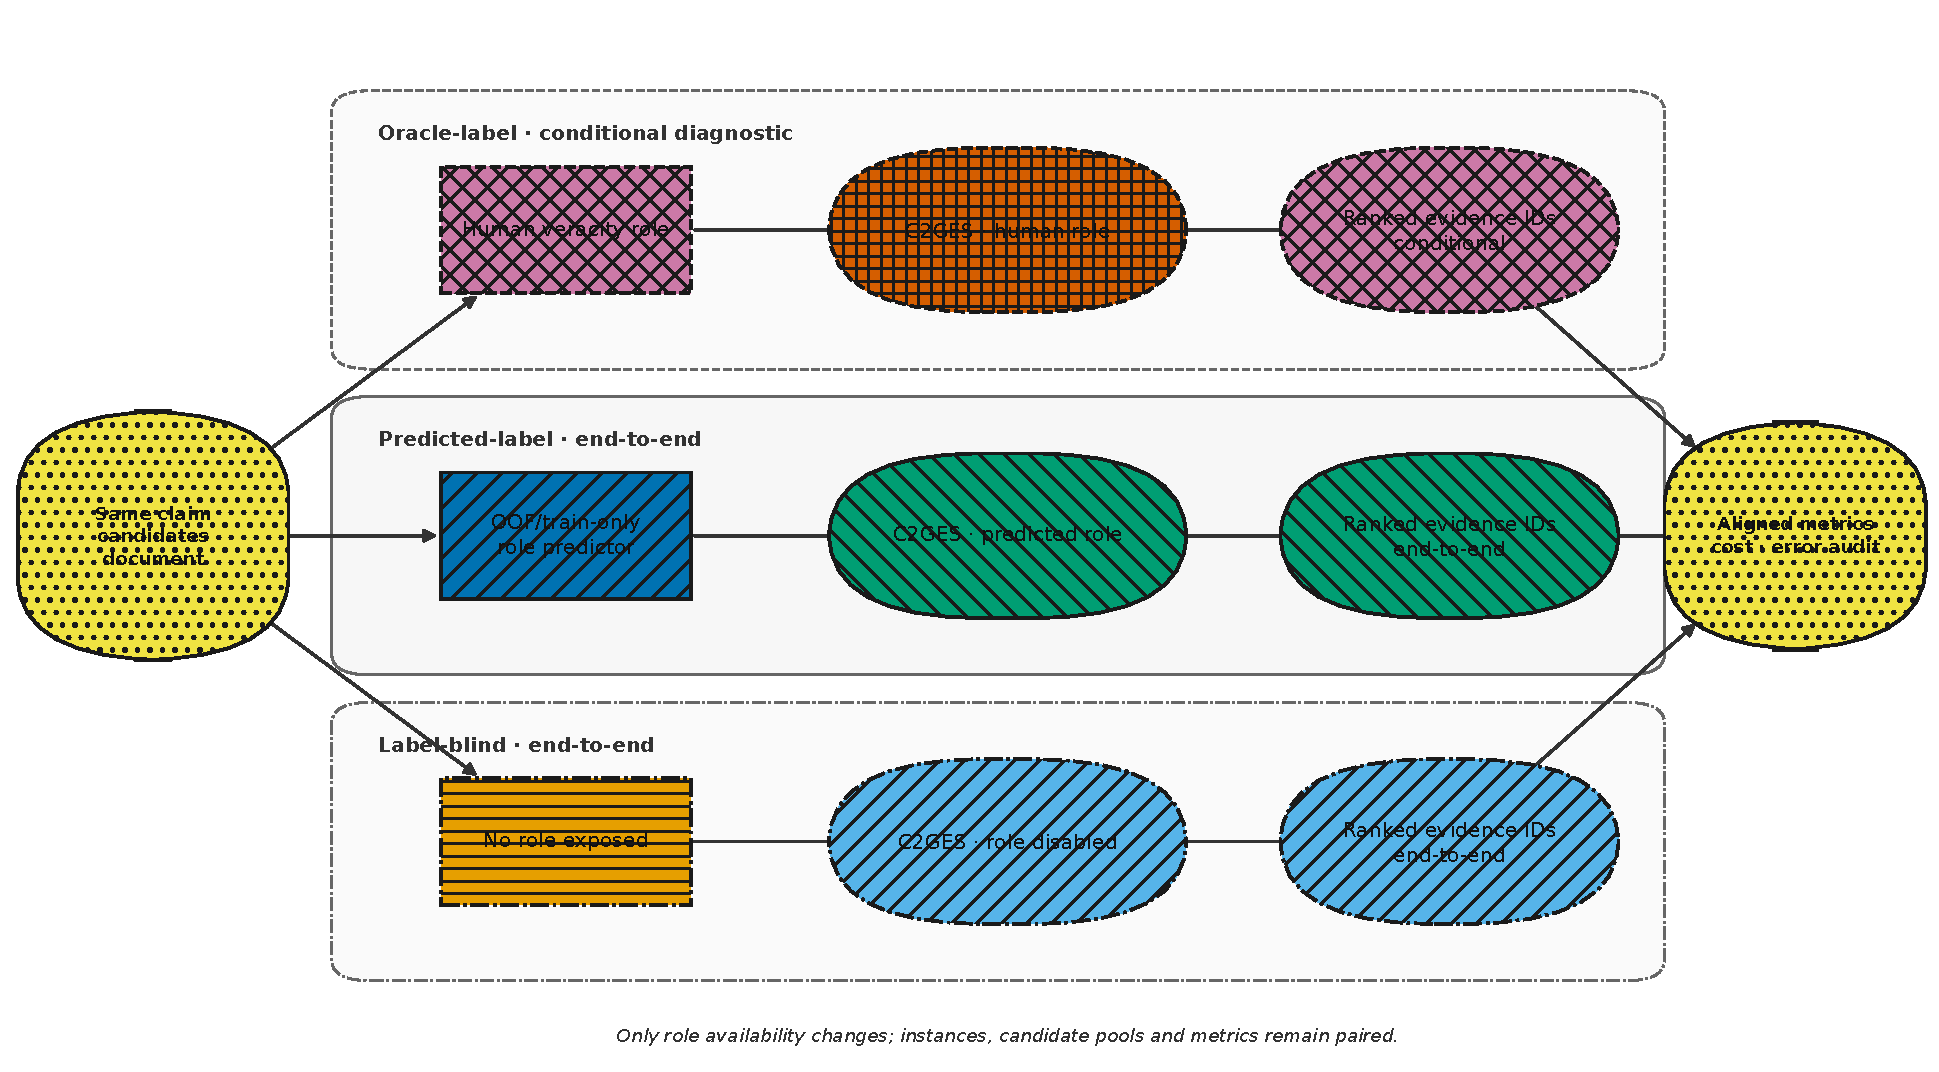
\includegraphics[width=0.96\textwidth]{figures/frameworks/c2_f01_three_protocols.pdf}
\caption{Three-protocol contract. Oracle-label is a privileged-label conditional sensitivity diagnostic; predicted-label and label-blind are end-to-end variants. Gold evidence enters training and evaluation but never candidate scoring.}\label{fig:protocols}
\end{figure}

\begin{figure}[H]
\centering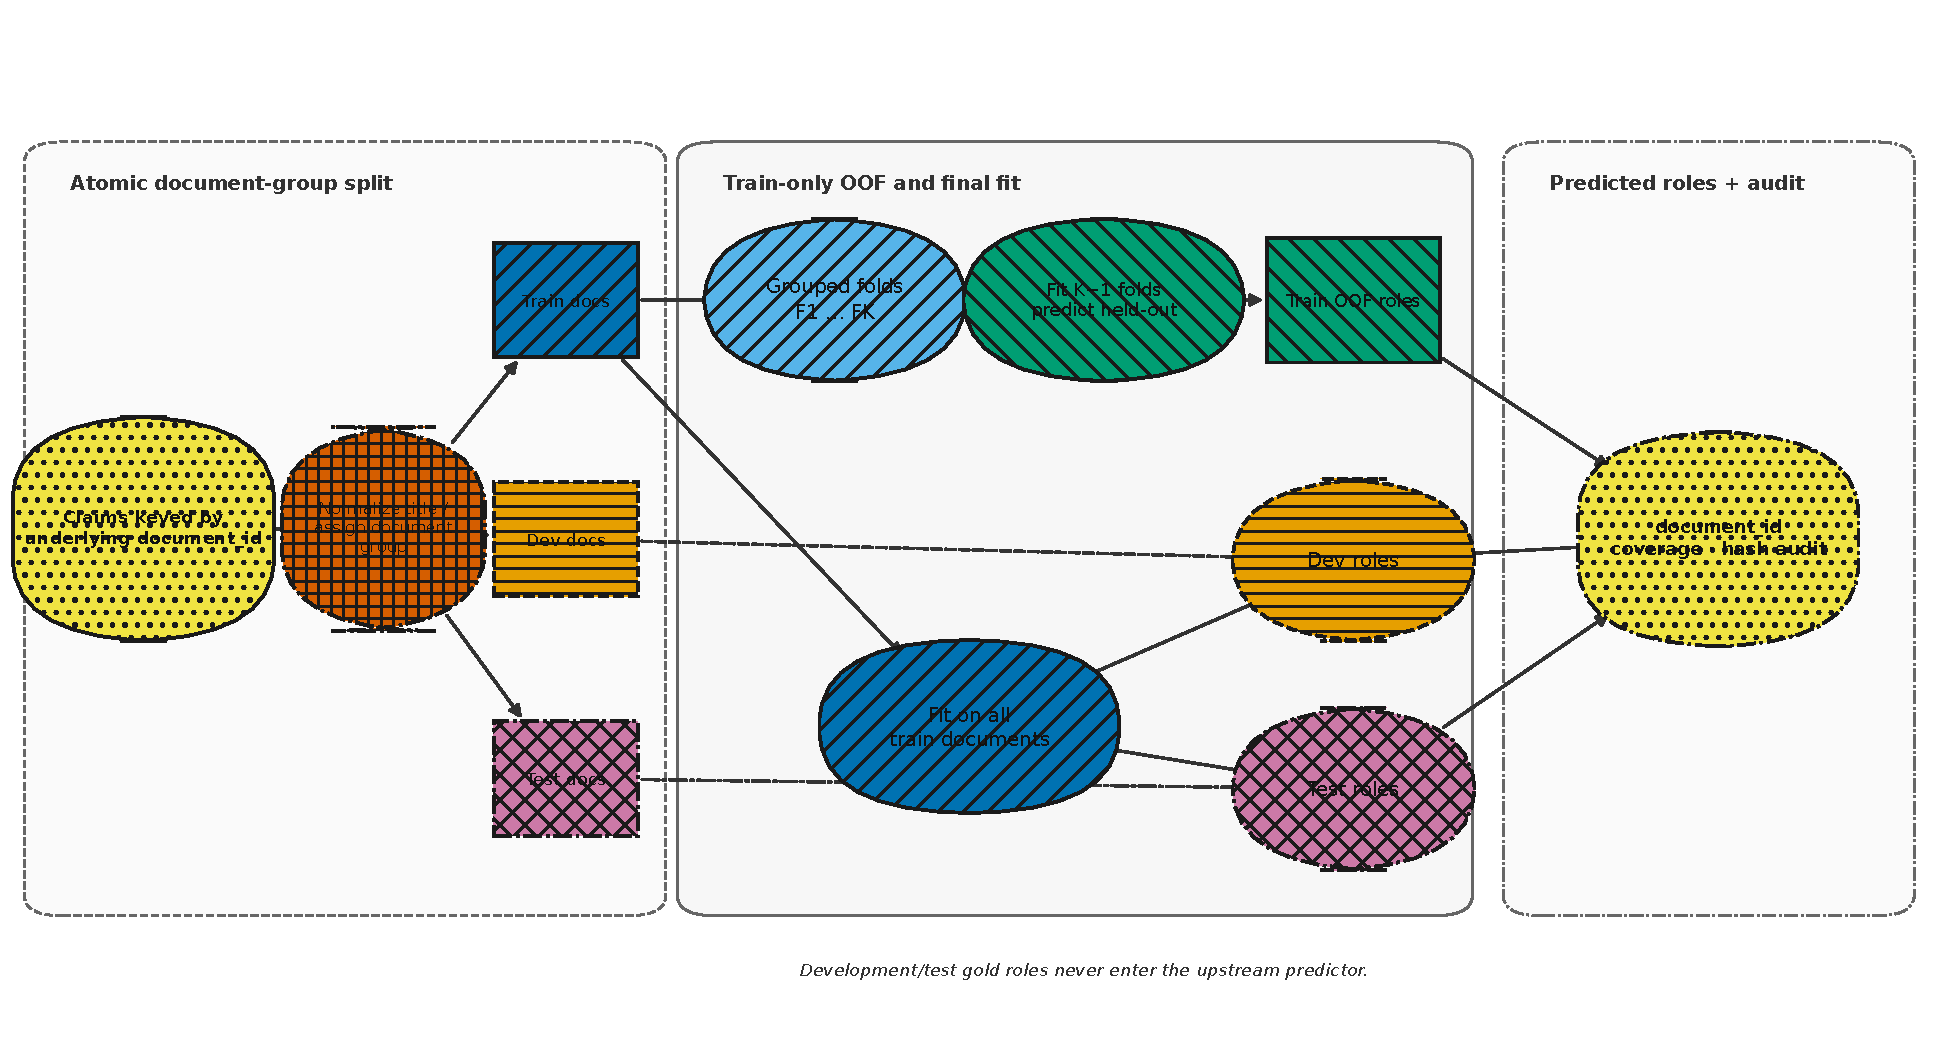
\includegraphics[width=0.96\textwidth]{figures/frameworks/c2_f02_oof_document_split.pdf}
\caption{Document-grouped splitting and out-of-fold role construction. Each source document is atomic, and each training role prediction comes from a model not fitted on that document.}\label{fig:oof}
\end{figure}

The upstream classifier is part of the predicted-label workflow, so its errors are not replaced by oracle roles. Table~\ref{tab:upstream} reports its frozen metrics. Test accuracy is \UpstreamTestAccuracy{} and macro-F1 is \UpstreamTestMacroFOne{}.

\begin{table}[H]
\caption{Upstream role-prediction performance. All values are generated from the immutable metrics artifact.}\label{tab:upstream}
\centering\resizebox{\textwidth}{!}{\begin{tabular}{llrrr}
\toprule
Partition & Prediction scheme & Accuracy & Balanced accuracy & Macro-F1 \\
\midrule
Train & Document-grouped OOF & 0.774 & 0.736 & 0.736 \\
Development & Train-only model & 0.793 & 0.759 & 0.761 \\
Test & Train-only model & 0.800 & 0.762 & 0.765 \\
\bottomrule
\end{tabular}
}
\end{table}

\subsection{Interpretable Mixture Reranker}
The frozen sentence encoder maps claims and candidates to $h_i^q$ and $h_{ij}$. The query channel $Q_{ij}$ equally combines within-document normalized embedding cosine similarity and TF--IDF cosine similarity. The role channel concatenates the sentence, claim, and role representations:
\begin{equation}
R_{ij}=\sigma\!\left(W_2\operatorname{ReLU}\left[W_1(h_{ij}\oplus h_i^q\oplus e(r_i))+b_1\right]+b_2\right).
\end{equation}
The local channel $G_{ij}$ smooths query salience over sentence position. It is a positional consistency prior, not an inferred causal graph.

All query-channel normalizations are computed within the candidate document. Scores therefore represent relative salience for one claim and should not be compared as calibrated probabilities across documents. A constant channel maps to zero rather than being divided by a zero range. Semantic and lexical terms are combined before the final mixture, keeping query relevance as one identifiable source in the downstream trace.

The role head receives frozen sentence and claim representations plus a learned embedding of the protocol-specific role. A shallow nonlinear transformation returns a bounded candidate score. Freezing the encoder reduces compute and makes across-seed changes easier to attribute to the head and mixture, but it also limits task adaptation. It is a reproducibility choice for this study, not a claim of optimality.

The local channel averages nearby query salience with distance-decaying weights and then normalizes within the document. It can promote a sentence near other relevant sentences, reflecting the common writing pattern in which context and evidence occupy a short neighborhood. It cannot establish event direction or physical propagation. Candidate traces therefore label the value as positional consistency rather than causal structure.

The final score is an additive positive mixture,
\begin{equation}
S_{ij}=w_QQ_{ij}+w_RR_{ij}+w_GG_{ij},\qquad w_m\geq 0,\quad \sum_m w_m=1.
\end{equation}
Mixture parameters are transformed to positive values, combined with predefined component floors, and renormalized. These floors make channel presence auditable but also constrain the optimum; consequently, fitted weight magnitudes are not treated as causal importance estimates.

Positivity makes a trace easier to interpret because every channel can only add support to a candidate. The trade-off is reduced flexibility: the model cannot learn that a high channel value should suppress a sentence, and a floor can keep an unhelpful component present. The role floor is especially relevant because the predefined role-effect criterion was not met. A future no-floor experiment must be prospectively specified as a new comparison rather than used retrospectively to replace the frozen outcome.

For positive evidence candidates $P_i$ and remaining candidates $N_i$, training uses pairwise softplus ranking loss,
\begin{equation}
\mathcal{L}_{\mathrm{rank},i}=\frac{1}{|P_i||N_i|}\sum_{p\in P_i}\sum_{n\in N_i}\log\!\left(1+\exp(S_{in}-S_{ip})\right),
\end{equation}
The implemented total loss is
\begin{equation}
\mathcal{L}_{i}=\mathcal{L}_{\mathrm{rank},i}(S)+0.5\,\mathcal{L}_{\mathrm{rank},i}(R),
\end{equation}
where $R$ is the sigmoid-bounded role-head score and both terms enumerate every positive--negative pair within an instance. The encoder snapshot, configuration, code hashes, upstream-role ledger, predictions, component traces, and resource logs are retained for each run.

The pairwise objective compares annotated evidence sentences with non-evidence candidates from the same document, matching the relative ordering required by top-$K$ inference. The auxiliary loss encourages the role head itself to distinguish positives from negatives. It does not guarantee that role identity supplies unique information: if claim and sentence representations already encode the useful distinction, predicted and blind protocols can remain empirically indistinguishable.

At inference, all channels are computed, combined, sorted, and truncated at the requested budget. The ledger retains selected identifiers, evaluator-only gold identifiers, role provenance, candidate scores, seed, protocol, cutoff, and configuration. These fields allow an aggregate result to be recomputed and a disputed item to be inspected without retraining.

\begin{table}[H]
\caption{Frozen downstream implementation choices, generated from a hash-bound implementation contract checked against the executable source.}\label{tab:implementation}
\centering\small\begin{tabular}{>{\raggedright\arraybackslash}p{0.16\textwidth}>{\raggedright\arraybackslash}p{0.35\textwidth}>{\raggedright\arraybackslash}p{0.37\textwidth}}
\toprule
Element & Frozen choice & Implementation detail \\
\midrule
Encoder & all-MiniLM-L6-v2; frozen; batch 64 & snapshot 1110a243...; tree SHA-256 091de8e3... \\
Role head & role embedding = encoder dimension; hidden 256 & ReLU; dropout 0.1; sigmoid output; 3 role IDs \\
Query channel & 0.5 normalized embedding cosine + 0.5 normalized TF--IDF cosine & per-document word (1,2)-grams; min\_df=1 \\
Local channel & all other sentences; exp(-|i-j|/3) & query-salience proxy; no finite window \\
Mixture & floors (0.35, 0.25, 0.05); raw init (0.8, 0.7, 0.2) & softplus + 1e-3; normalize, add floors, renormalize \\
Loss & pairwise softplus on total score + 0.5 pairwise softplus on role score & all positive--negative pairs within an instance \\
Optimization & Adam; lr 0.001; weight decay 0; 4 epochs & PyTorch defaults; one optimizer step per document-instance \\
Selection & development F1 at K=3; strict improvement & earliest epoch retained on a tie; descending argsort at inference \\
Randomness & Python, NumPy, and PyTorch seeded & training-instance shuffle each epoch; CPU execution \\
Normalization & within-document min--max & range below 1e-12 maps to all zeros \\
\bottomrule
\end{tabular}

\end{table}

\subsection{Five-Seed Statistical Protocol}
The first seed (2026) was completed and inspected during pipeline development. Before seeds 2027--2030 were run, the endpoint, protocols, evidence budgets, aggregation rule, and decision criteria were fixed in a dated manifest. The reported analysis includes the pilot seed rather than selecting only the four prospectively executed runs. This timing limits a fully prospective interpretation, but it preserves the complete run history and prevents favorable seed selection.

The aggregation uses \SeedCount{} downstream training seeds, cutoffs $K\in\{\EvalCutoffs\}$, \TrainingEpochs{} epochs, learning rate \LearningRate{}, and \BootstrapSamples{} bootstrap replicates. The MiniLM encoder identifier is \texttt{\EncoderModel}; its exact snapshot reference is \texttt{1110a243...b4d41} with tree SHA-256 \texttt{091de8e3...4f81}. Learned protocols are fitted independently per downstream seed. BM25 is deterministic and evaluated on the identical candidate pool.

For predicted set $\widehat E_i^{(K)}$, per-instance precision, recall, and F1 are computed from sentence-ID overlap with $E_i$. Macro evidence F1 is the primary reported metric. Paired uncertainty resamples the \TestDocuments{} test source documents and includes every item from each sampled document. The hierarchical interval additionally samples training seeds. The role-effect criterion requires a positive predicted-label minus label-blind mean and both seed-level and hierarchical intervals to exclude zero. This rule was fixed before the remaining four seeds were executed and before the five-seed aggregation.

Macro averaging gives every claim equal weight. Per-item precision is the share of selected identifiers that are annotated, recall is the share of annotated identifiers returned, and F1 is their harmonic mean with a defined zero for an empty denominator. Because changing the output budget alters the precision denominator and attainable recall, different cutoffs are distinct operating points rather than repeated estimates of one invariant performance value.

Paired contrasts preserve item and document assignments between systems. The hierarchical procedure uses a deterministic NumPy RNG seed defined in the aggregator for each contrast. It samples five downstream seeds with replacement; within each sampled seed it samples that seed's document clusters with replacement, repeats a duplicated cluster with all of its claims, pools the resulting claim-level differences, and takes their mean. Thus the estimand is instance-weighted rather than equally weighted by document. The reported 95\% interval is the 2.5th--97.5th percentile interval over \BootstrapSamples{} draws, whose finite Monte Carlo count limits endpoint precision. The seed-level interval is a two-sided $t$ interval over the five paired seed means. Both interval lower bounds, as well as a positive mean, are required by every positive-effect criterion. Resampling documents preserves within-page dependence \cite{cameron2008bootstrap}.

The frozen aggregator reports raw paired $t$-test and exact sign-flip $p$-values, but the decision criteria use neither value: they use the positive mean and the two unadjusted interval lower bounds just defined. No Holm correction or other multiplicity adjustment was implemented for this primary analysis, so none is claimed. Cutoff and protocol comparisons form a correlated descriptive matrix; a favorable secondary cell cannot reverse the predefined primary role decision.

BM25 supplies one deterministic result rather than artificial seed variation. Comparison uncertainty arises from paired documents and the learned systems' downstream seeds. A point estimate meets the positive-effect criterion only when its mean is positive and both the seed-level $t$ interval and hierarchical percentile interval are wholly above zero; meeting it at one budget does not imply meeting it elsewhere.

\subsection{Crossed Upstream--Downstream Seed Sensitivity}
The main five-seed analysis reuses one upstream role-prediction ledger, so its uncertainty does not include variation from refitting the upstream classifier. A separately hash-bound sensitivity experiment rebuilds document-grouped out-of-fold roles with upstream seeds 3101--3105. For each upstream ledger, the selector is trained with downstream seeds 2026--2030, producing a crossed $5\times5$ matrix of 25 full pipelines. The data partitions, encoder snapshot, training limits, four-epoch schedule, learning rate, evidence budgets, and exact sentence-ID metric remain unchanged. Completion requires five successful upstream builds, 25 successful downstream runs, and 25 prediction ledgers of exactly 54,000 rows each.

The primary sensitivity estimand is claim-weighted macro F1 for the full predicted-role model at $K=3$, averaged over the 25 cells. A two-way method-of-moments decomposition reports descriptive contributions from the five fixed upstream seeds, five fixed downstream seeds, and their interaction/residual. It is not a population random-effects model. A separate 10,000-draw procedure resamples the 145 test documents while preserving every complete upstream--downstream cell; its percentile range measures document-composition sensitivity rather than population confidence. The archived \texttt{no\_role} mode remains an inference ablation and is not described as a separately retrained label-blind model.

Writing $MS_U$, $MS_D$, and $MS_E$ for the usual two-way mean squares with 4, 4, and 16 degrees of freedom, respectively, and $n_U=n_D=5$, the reported components are
\begin{equation}
\widehat{\sigma}_U^2=\max\!\left(0,\frac{MS_U-MS_E}{n_D}\right),\qquad
\widehat{\sigma}_D^2=\max\!\left(0,\frac{MS_D-MS_E}{n_U}\right),\qquad
\widehat{\sigma}_{UD+E}^2=MS_E.
\end{equation}
The nonnegative truncation is part of the descriptive estimator; it is not evidence that a true population variance equals zero.

\subsection{Reproducibility and Failure Controls}
The registry freezes data and hashes, encoder identity and snapshot, training configuration, seeds, cutoffs, resampling count, and overwrite policy. A completed run is accepted only when its summary, configuration, provenance, predictions, resource log, and standard streams are present and mutually consistent. Cartesian checks verify every expected protocol--seed--item--cutoff record. Resume operations do not silently replace completed evidence.

Aggregation uses only indexed runs that satisfy the frozen configuration and integrity checks. Tables are recomputed from complete prediction ledgers, source hashes are attached, and figures are rendered from the resulting tabular release. The reproducibility manifest covers code, environment information, converted data, the upstream role ledger and model, all 15 downstream configurations and checkpoints, the exploratory comparisons, and the prospective structural-ablation package. The verification script also checks the decompressed hash, byte count, and line count of the compressed prediction payload. These controls establish numerical reproducibility for the reported results; long-term accessibility additionally requires deposit in a permanent public archive.

Failure reporting is part of the result. A missing seed, incomplete ledger, hash mismatch, or protocol inconsistency would block the primary table. Resource claims are bounded as well: wall time covers the full CPU script, while sampled resident memory is not a precise measure of accelerator use or transient allocation peaks.

\begin{figure}[H]
\centering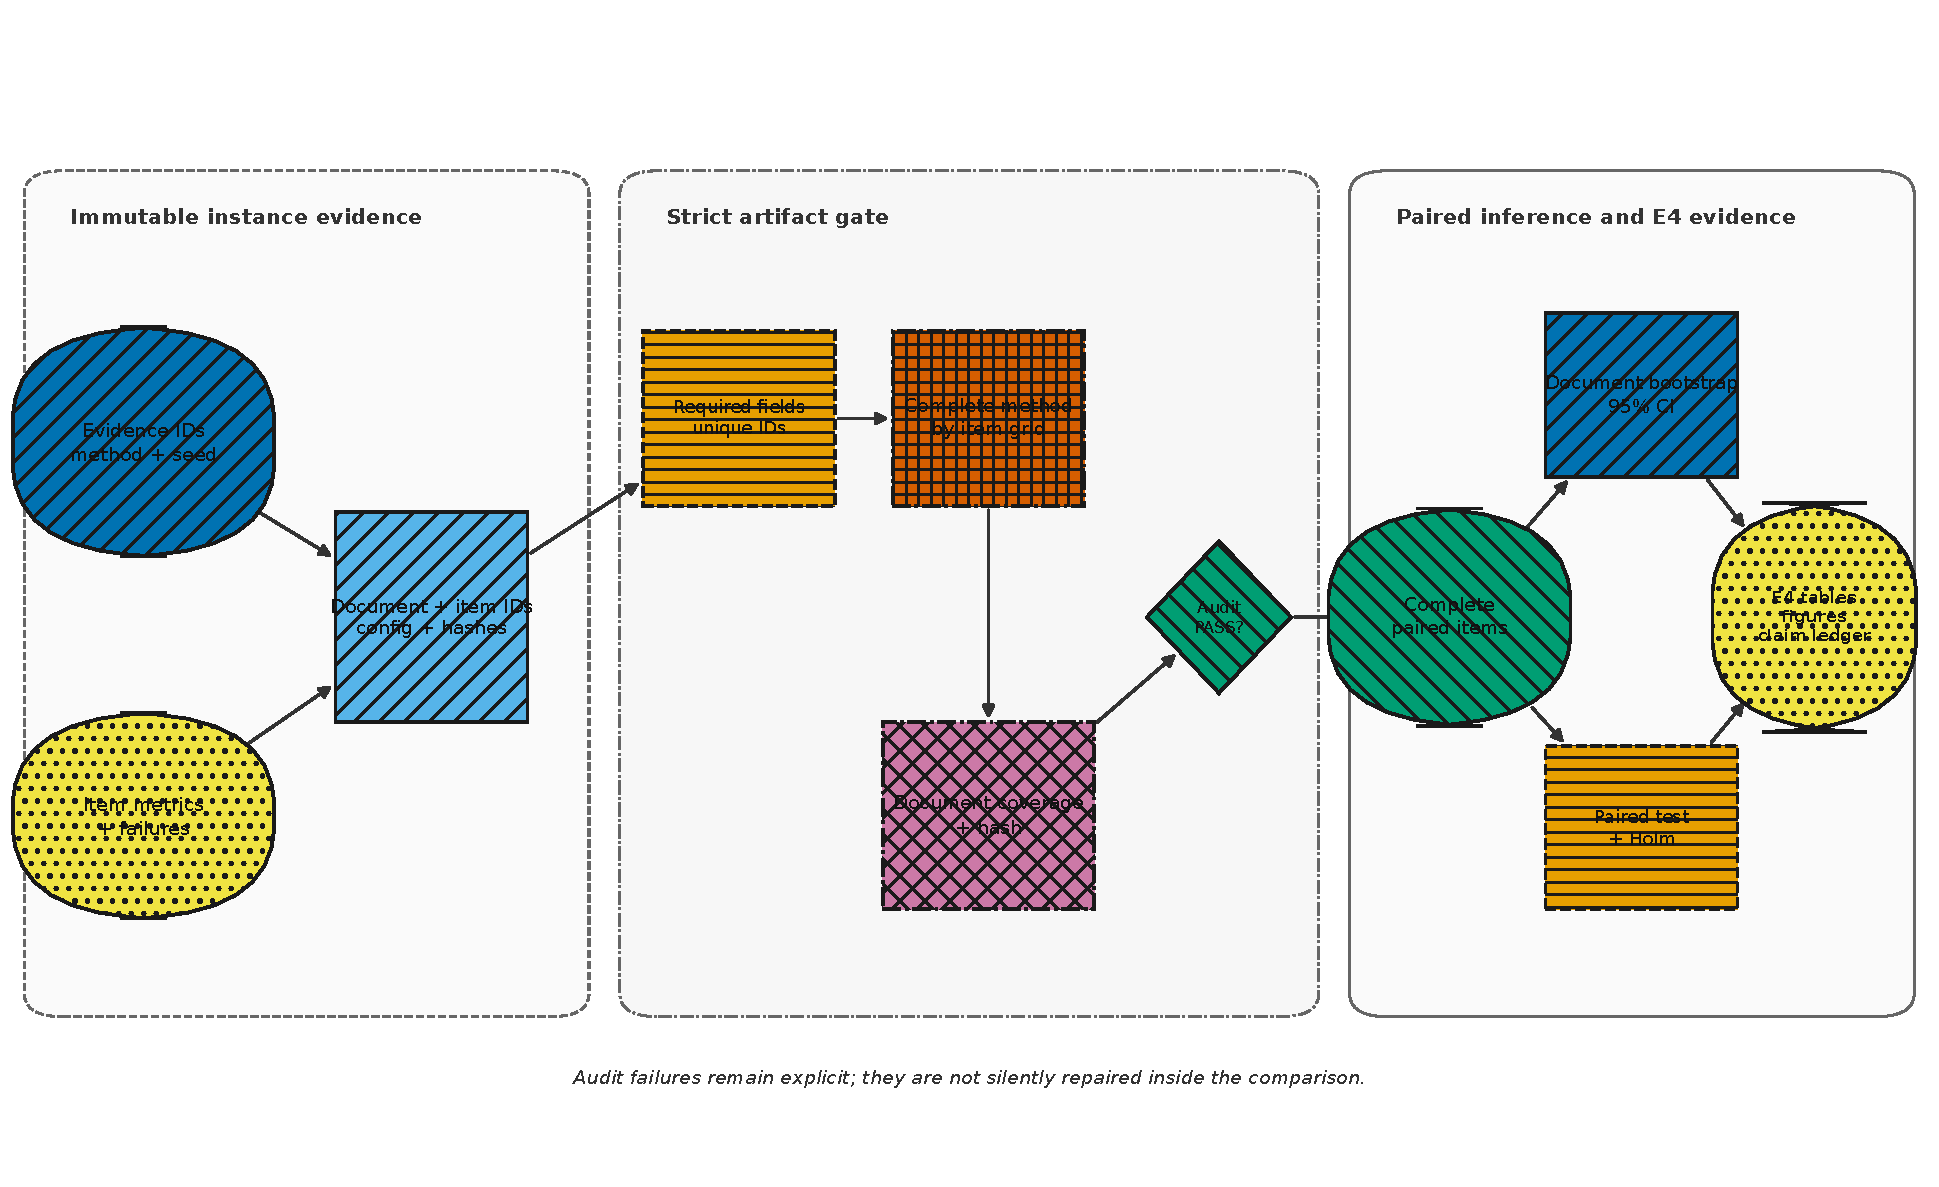
\includegraphics[width=0.96\textwidth]{figures/frameworks/c2_f03_evidence_audit_bootstrap.pdf}
\caption{Evidence-ledger audit and paired document-cluster analysis. Completeness, hashes, and protocol provenance are checked before statistical contrasts are released.}\label{fig:audit}
\end{figure}

\section{Results}
\subsection{Audit and Main Performance}
All \SuccessfulRuns{} protocol--seed runs succeeded; the evidence audit passed \AuditChecks{} checks with \AuditFailures{} failures. The 15 source ledgers contain 810,000 rows across all recorded modes (54,000 per run). The primary release retains \CanonicalPredictionRows{} full-model and BM25 rows (12,000 per run: 1,500 test instances at four cutoffs for each of the two modes). Table~\ref{tab:main} reports this predefined scope. Oracle-label values are marked as conditional and must not be interpreted as deployed results.

\begin{table}[H]
\caption{Five-seed evidence F1 by role-provenance protocol and budget. SD is the sample standard deviation across downstream seeds. Every displayed criterion requires a positive mean and positive lower bounds for both the seed-level $t$ interval and hierarchical percentile interval. These predefined cutoff-specific gates are not multiplicity-adjusted and do not support a blanket superiority claim; complete intervals are retained in the effects artifact. $\dagger$ denotes a conditional, non-end-to-end protocol.}\label{tab:main}
\centering\resizebox{\textwidth}{!}{\begin{tabular}{llrrrr}
\toprule
System & $K$ & Mean F1 & SD & $\Delta$ vs. BM25 & Criterion \\
\midrule
Oracle-label$^{\dagger}$ & 1 & 0.6705 & 0.0050 & -0.0289 & Not met \\
Oracle-label$^{\dagger}$ & 3 & 0.4926 & 0.0015 & +0.0062 & Met \\
Oracle-label$^{\dagger}$ & 5 & 0.4160 & 0.0009 & +0.0051 & Met \\
Oracle-label$^{\dagger}$ & 10 & 0.3563 & 0.0001 & +0.0033 & Met \\
Predicted-label & 1 & 0.6688 & 0.0051 & -0.0306 & Not met \\
Predicted-label & 3 & 0.4920 & 0.0021 & +0.0056 & Met \\
Predicted-label & 5 & 0.4150 & 0.0007 & +0.0041 & Met \\
Predicted-label & 10 & 0.3563 & 0.0002 & +0.0033 & Met \\
Label-blind & 1 & 0.6677 & 0.0021 & -0.0317 & Not met \\
Label-blind & 3 & 0.4910 & 0.0021 & +0.0046 & Not met \\
Label-blind & 5 & 0.4154 & 0.0006 & +0.0045 & Met \\
Label-blind & 10 & 0.3560 & 0.0003 & +0.0031 & Met \\
BM25 & 1 & 0.6994 & 0.0000 & +0.0000 & Reference \\
BM25 & 3 & 0.4864 & 0.0000 & +0.0000 & Reference \\
BM25 & 5 & 0.4109 & 0.0000 & +0.0000 & Reference \\
BM25 & 10 & 0.3530 & 0.0000 & +0.0000 & Reference \\
\bottomrule
\end{tabular}
}
\end{table}

At the smallest budget, BM25 reaches \BMKOneFOne{} and every learned protocol is lower. At the primary budget, predicted-label reaches \PredKThreeFOne{} $\pm$ \PredKThreeSD{}, compared with \BMKThreeFOne{} for BM25. Its difference, \PredVsBMKThreeDelta{}, has hierarchical interval \PredVsBMKThreeCI{} and passes the cutoff-specific positive gate. This local result does not justify blanket superiority because the smallest-budget comparison is negative and not all systems pass at every cutoff.

The cutoff trajectory is consistent across the three learned protocols: macro F1 decreases as more sentences are returned because precision is divided over a larger packet, while recall opportunity increases. The scientific question is therefore not whether a larger cutoff produces a larger F1, but which ranking is most useful at the reading budget an application can afford. A one-sentence answer favors lexical concentration in this benchmark. At moderate budgets, selected protocol--BM25 differences are positive under the predefined cutoff-specific comparison; this observation does not identify a causal channel or establish recovery beyond the exact sentence-ID endpoint.

The similar trajectories of oracle, predicted, and blind variants are themselves informative. If role identity were a strong and unique selector signal, one would expect stable separation between these curves, especially between oracle and blind. Instead, differences are small relative to across-seed and across-document uncertainty. This contrast supports only the narrow conclusion that changing role provenance did not reliably change the full reranker here; it does not identify which remaining channel caused the system-level behavior.

Source ledgers also contain diagnostic modes that were not part of the primary full-model--BM25 comparison. We therefore defined a finite post-primary analysis of all nine existing modes, all five seeds, three role protocols, and $K\in\{1,3,5,10\}$ before examining the complete comparison family. Because these predictions already existed and some individual modes had been inspected, the analysis is exploratory rather than prospective and does not alter the predefined primary decisions. At label-blind $K=3$, full-model F1 was 0.4910; mode-minus-full differences ranged from $-0.0858$ (LexCue) to $-0.0006$ (no-local). Five-seed exact sign-flip tests have a minimum attainable two-sided $p=0.0625$, and Holm adjustment across the eight frozen comparisons yielded no positive finding. The corrected intervals resample documents and pool every claim and complete seed bundle in each sampled cluster, matching the claim-weighted point estimand; independent recomputation exactly reproduced every stored interval. Figure~\ref{fig:exploratory} reports every primary contrast, and the hash-bound package retains all 108 cells and all multiplicity families. A cross-encoder and a true no-floor ablation were not part of this exploratory family and were evaluated separately.

\begin{figure}[H]
\centering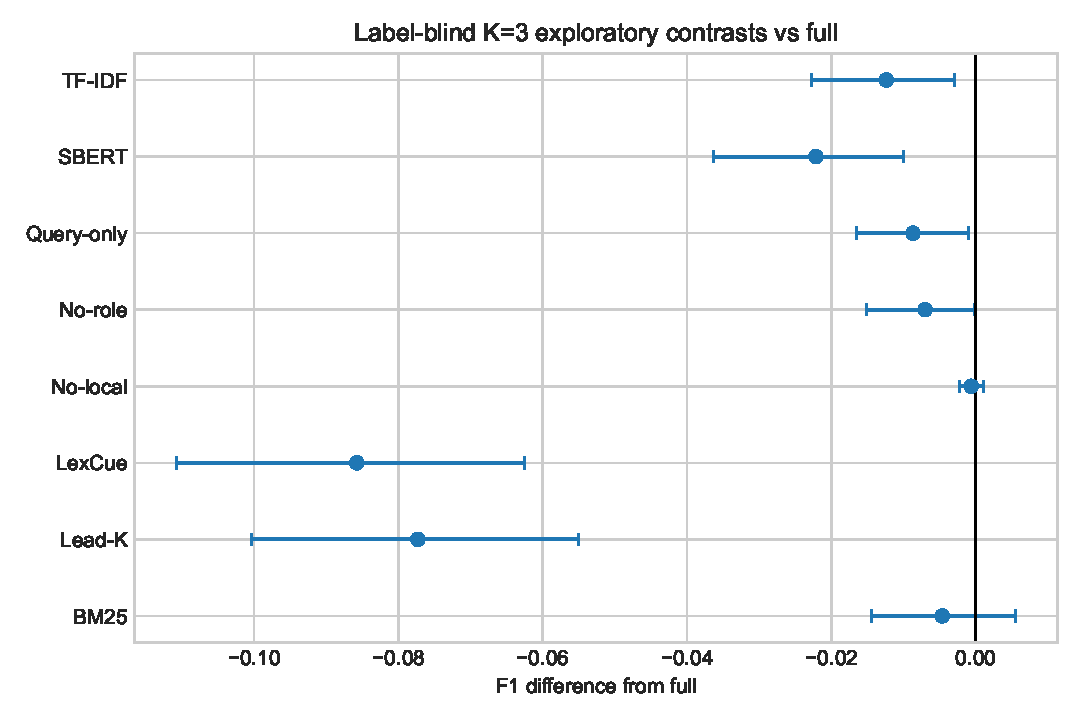
\includegraphics[width=0.82\textwidth]{figures/results/fig06_exploratory_forest.pdf}
\caption{Post-primary exploratory label-blind comparisons at $K=3$. Points are mode-minus-full macro evidence-F1 differences; intervals are paired document-cluster bootstrap intervals. All eight frozen comparisons are shown, and exact five-seed tests are Holm-adjusted as one family. This panel does not modify the predefined role-effect or BM25 decisions.}\label{fig:exploratory}
\end{figure}

The missing structural and neural comparisons were specified in a separate prospective protocol before execution. This experiment retains the same documents, candidates, exact-ID metric, and budgets, but restricts the primary estimand to deployment-valid label-blind $K=3$. True no-floor and structurally role-free models were retrained independently for all five seeds; the latter has no role-head parameters and exactly zero role weight. A zero-shot cached cross-encoder was run from revision \texttt{c5ee24cb...b1df96625c6b8}. Table~\ref{tab:addon} reports all seven frozen arm-minus-full comparisons. Cross-encoder minus full was $+0.0102$ with a claim-weighted document-cluster interval of $[+0.0007,+0.0200]$, but its Holm-adjusted $p=0.1877$ did not support a positive claim. True no-floor minus full was $-0.0040$ with interval $[-0.0090,+0.0008]$; true no-role minus full was $-0.0080$ with interval $[-0.0162,-0.0008]$, also without a Holm-adjusted finding. These prospective results provide stronger method comparisons while leaving both primary decisions unchanged.

\begin{table}[H]
\caption{Prospectively specified comparisons at label-blind $K=3$. Point estimates and intervals use the same claim-weighted estimand; Holm adjustment covers all seven frozen arm-minus-full contrasts.}\label{tab:addon}
\centering\resizebox{0.93\textwidth}{!}{\input{generated/table_structural_neural_contrasts.tex}}
\end{table}

\subsection{Independent BGE Strong-Baseline Comparison}
A separately specified evaluation compared the frozen zero-shot \nolinkurl{BAAI/bge-reranker-base} snapshot (revision \texttt{2cfc18c...768a70}) with full \cges{}, BM25, and the MiniLM cross-encoder on the same 1,500 FEVER test claims and 145 source-document clusters. BGE received only a claim--candidate-sentence pair, without a veracity label or gold evidence. The candidate pool, exact sentence-ID metric, and $K\in\{1,3,5,10\}$ budgets were unchanged. Full \cges{} was averaged over its complete five-seed bundle at claim level; the other three methods were deterministic single runs.

The primary endpoint was claim-weighted evidence F1 at $K=3$. For each BGE-minus-comparator contrast, a 10,000-draw document-cluster bootstrap quantified sensitivity to the composition of the observed test documents, and a 100,000-sample two-sided document-cluster sign-flip test supplied the raw $p$-value. Holm adjustment covered exactly the three contrasts in Table~\ref{tab:bge}. These percentile ranges are composition-sensitivity intervals, not population confidence intervals. They are conditional on the complete frozen five-seed \cges{} bundle: training seeds are averaged at claim level rather than resampled as an additional uncertainty source.

\begin{table}[H]
\caption{Frozen zero-shot BGE comparisons on human-annotated FEVER evidence at $K=3$. Differences are BGE minus comparator. Intervals describe sensitivity to resampling the observed document composition; Holm adjustment covers the three displayed contrasts.}\label{tab:bge}
\centering\resizebox{0.88\textwidth}{!}{\input{generated/table_bge_contrasts.tex}}
\end{table}

BGE attained F1 values of 0.6112, 0.4890, 0.4169, and 0.3593 at $K=1,3,5,10$, respectively. At the primary budget, its difference from full \cges{} was $-0.0021$ with composition-sensitivity interval $[-0.0137,+0.0090]$; the corresponding difference from BM25 was $+0.0026$ with interval $[-0.0116,+0.0162]$. Although the interval for BGE minus MiniLM was wholly negative, its randomization result did not meet the prespecified family criterion after Holm adjustment ($p_{\mathrm{Holm}}=0.1710$). Thus none of the three BGE comparisons supports a promoted difference. This finding concerns zero-shot ranking on human-annotated FEVER evidence only.

The BM25 comparison illustrates why a single operating point can mislead. Reporting only the primary cutoff would omit the setting in which the deterministic lexical method clearly leads. Reporting only the smallest cutoff would omit the settings in which selected learned variants pass a positive paired gate. The complete cutoff table is thus part of the claim boundary, and the figure uses distinct markers and line styles so the conditional oracle is not visually merged with deployable systems.

\begin{figure}[H]
\centering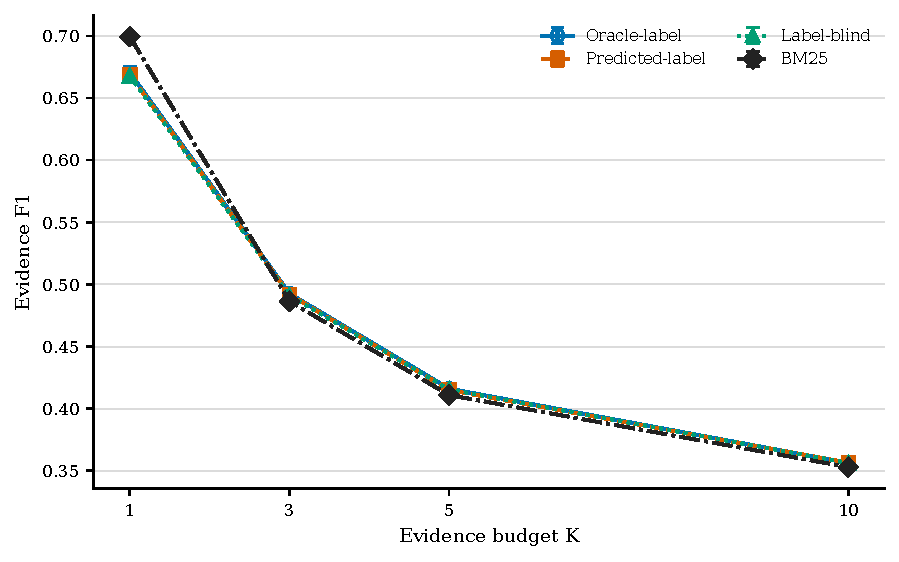
\includegraphics[width=0.92\textwidth]{figures/results/fig01_k_sensitivity_f1.pdf}
\caption{Five-seed results, comprising one pilot seed and four prospectively specified continuation seeds. Error bars denote one sample SD. Oracle-label is conditional; neither the predefined role-effect criterion nor the criterion for superiority across budgets was met.}\label{fig:k}
\end{figure}

\subsection{Role-Effect Decision}
Table~\ref{tab:role} and Figure~\ref{fig:role} directly test whether the role source changes evidence ranking. At the primary budget, predicted-label minus label-blind is \RoleKThreeDelta{}. The seed-level interval is \RoleKThreeTCI{} and the hierarchical interval is \RoleKThreeHierCI{}; both include zero. Every predefined role contrast at the primary budget likewise crosses zero. Role conditioning is therefore a tested mechanism without a supported primary effect in this experiment.

The conclusion is based on uncertainty as well as magnitude. The positive mean for predicted minus blind is too small to distinguish from zero under either seed-level or hierarchical inference. Oracle comparisons also fail the same primary gate. Because the oracle has access to strictly more privileged information, its failure to separate reliably from blind strengthens the scoped interpretation that binary veracity is not a decisive ranking input in this document-conditioned setup.

Other cutoffs do not reverse the predefined conclusion. The direction changes for some contrasts and the hierarchical intervals include zero. Highlighting the most favorable observed cell would therefore be a post hoc selection over a family of correlated comparisons. We retain the full contrast matrix and report every role criterion explicitly. The negative finding also guards against reading the role mixture weight as proof: a constrained model can allocate weight to a channel even when replacing its input with a constant yields no stable loss in test F1.

Upstream role prediction is adequate for evaluating a realistic two-stage path but is imperfect, as shown in Table~\ref{tab:upstream}. Prediction errors can attenuate a useful role signal, yet the oracle comparison does not show a reliable primary advantage either. It would therefore be premature to attribute the unsupported role effect solely to upstream error. More fine-grained application roles, stronger upstream modeling, and an unconstrained mixture are reasonable future hypotheses, each requiring a new prospectively specified test.

\begin{table}[H]
\caption{Paired role-source contrasts. Hierarchical intervals resample source documents within training seeds. Oracle contrasts are conditional.}\label{tab:role}
\centering\resizebox{\textwidth}{!}{\begin{tabular}{llrrr}
\toprule
Contrast & $K$ & Mean $\Delta$ & Hierarchical 95\% CI & Criterion \\
\midrule
Oracle$^{\dagger}$ $-$ predicted & 1 & +0.0018 & [-0.0023, 0.0061] & Not met \\
Oracle$^{\dagger}$ $-$ predicted & 3 & +0.0006 & [-0.0012, 0.0023] & Not met \\
Oracle$^{\dagger}$ $-$ predicted & 5 & +0.0011 & [-0.0002, 0.0023] & Not met \\
Oracle$^{\dagger}$ $-$ predicted & 10 & -0.0000 & [-0.0005, 0.0004] & Not met \\
Oracle$^{\dagger}$ $-$ blind & 1 & +0.0028 & [-0.0031, 0.0099] & Not met \\
Oracle$^{\dagger}$ $-$ blind & 3 & +0.0016 & [-0.0009, 0.0044] & Not met \\
Oracle$^{\dagger}$ $-$ blind & 5 & +0.0006 & [-0.0005, 0.0017] & Not met \\
Oracle$^{\dagger}$ $-$ blind & 10 & +0.0002 & [-0.0002, 0.0007] & Not met \\
Predicted $-$ blind & 1 & +0.0011 & [-0.0049, 0.0073] & Not met \\
Predicted $-$ blind & 3 & +0.0010 & [-0.0012, 0.0031] & Not met \\
Predicted $-$ blind & 5 & -0.0005 & [-0.0015, 0.0005] & Not met \\
Predicted $-$ blind & 10 & +0.0003 & [-0.0001, 0.0008] & Not met \\
\bottomrule
\end{tabular}
}
\end{table}

\begin{figure}[H]
\centering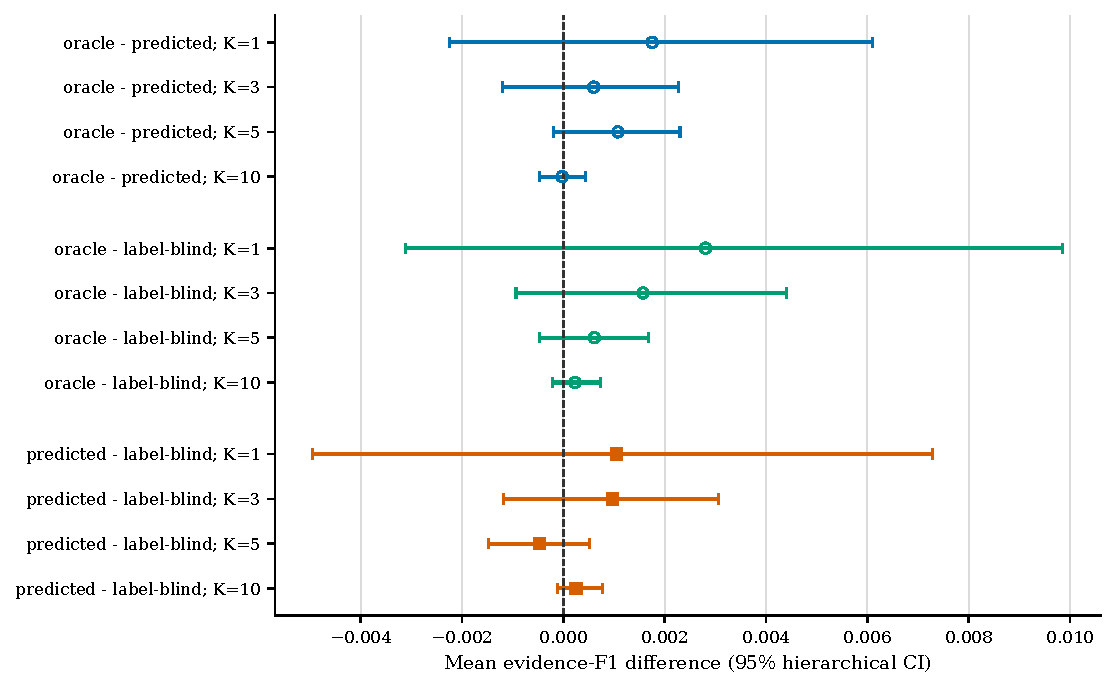
\includegraphics[width=0.92\textwidth]{figures/results/fig02_role_effect_forest.pdf}
\caption{Protocol differences with hierarchical seed/document intervals. Intervals crossing zero show that the predefined role-effect criterion was not met; oracle-label comparisons are conditional.}\label{fig:role}
\end{figure}

\subsection{Crossed Upstream--Downstream Seed Results}
The crossed sensitivity run completed all five upstream builds and all 25 downstream pipelines without dropping a cell. At the primary endpoint, the 25-cell grand mean was \UpstreamMatrixGrandFOne{}. Upstream-seed marginal means ranged from \UpstreamMatrixUpstreamRange{}, whereas downstream-seed marginal means ranged from \UpstreamMatrixDownstreamRange{}. The document-composition sensitivity interval was \UpstreamMatrixCompositionCI{}; by construction, this interval is not a population confidence interval. Table~\ref{tab:upstream-matrix} reports the descriptive variance decomposition together with these scale checks.

\begin{table}[H]
\caption{Crossed upstream--downstream seed sensitivity for the full predicted-role model at $K=3$. Variance components are descriptive method-of-moments quantities over the five fixed levels of each seed factor.}\label{tab:upstream-matrix}
\centering\begin{tabular}{lr}
\toprule
Quantity & Estimate \\
\midrule
Crossed upstream--downstream cells & 25 \\
Grand mean exact-ID F1 at $K=3$ & 0.4906 \\
Upstream-seed mean range & 0.4899--0.4913 \\
Downstream-seed mean range & 0.4879--0.4922 \\
Upstream variance component & 0.00000000 \\
Downstream variance component & 0.00000216 \\
Interaction/residual variance & 0.00000286 \\
Document-composition sensitivity interval & [0.4730, 0.5080] \\
\bottomrule
\end{tabular}

\end{table}

The upstream method-of-moments component was truncated at zero because its mean square was smaller than the interaction/residual mean square. The downstream and interaction/residual components were $2.16\times10^{-6}$ and $2.86\times10^{-6}$, respectively. Together with the narrower upstream marginal range, this indicates that upstream refitting was not the dominant source of variation among these chosen seeds. It does not imply that upstream-model uncertainty is universally absent. The experiment expands the original downstream-only seed analysis but does not turn five chosen upstream seeds into a population sample or alter the predefined role-effect and BM25 comparison families.

\subsection{Compute and Stability Diagnostics}
The measured wall time covers the full CPU training-and-evaluation script, not online per-query latency. Peak resident memory is sampled from the process tree and may miss short-lived peaks. Predicted-label has the additional upstream role stage, so small runtime differences should not be interpreted as a general efficiency advantage.

The resource table shows similar orders of magnitude across selector protocols, as expected from their shared encoder and architecture. It does not compare BM25 indexing cost, model download cost, hardware energy, or interactive latency. The compute--accuracy plot is therefore diagnostic rather than a definitive Pareto frontier. A deployment study should separate offline encoding and training from per-query scoring, report warm and cold caches, and measure the complete document ingestion path.

\begin{table}[H]
\caption{Full-script CPU wall time and sampled peak resident memory across seeds. Values are generated from the frozen resource logs.}\label{tab:runtime}
\centering\begin{tabular}{lrrrr}
\toprule
Protocol & Wall time (s) & SD (s) & Peak RSS (GiB) & SD (GiB) \\
\midrule
Oracle-label$^{\dagger}$ & 200.40 & 7.15 & 1.280 & 0.018 \\
Predicted-label & 204.99 & 11.41 & 1.270 & 0.033 \\
Label-blind & 200.40 & 4.96 & 1.274 & 0.017 \\
\bottomrule
\end{tabular}

\end{table}

\begin{figure}[H]
\centering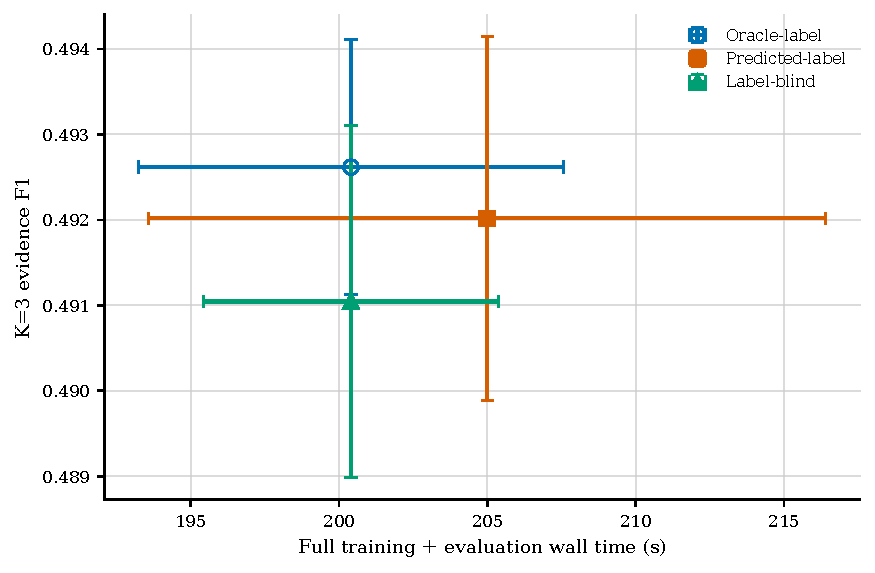
\includegraphics[width=0.82\textwidth]{figures/results/fig03_compute_accuracy_tradeoff.pdf}
\caption{Measured full-script CPU time against primary-budget F1. Error bars are one seed SD; the plot does not represent online latency.}\label{fig:compute}
\end{figure}

\begin{figure}[H]
\centering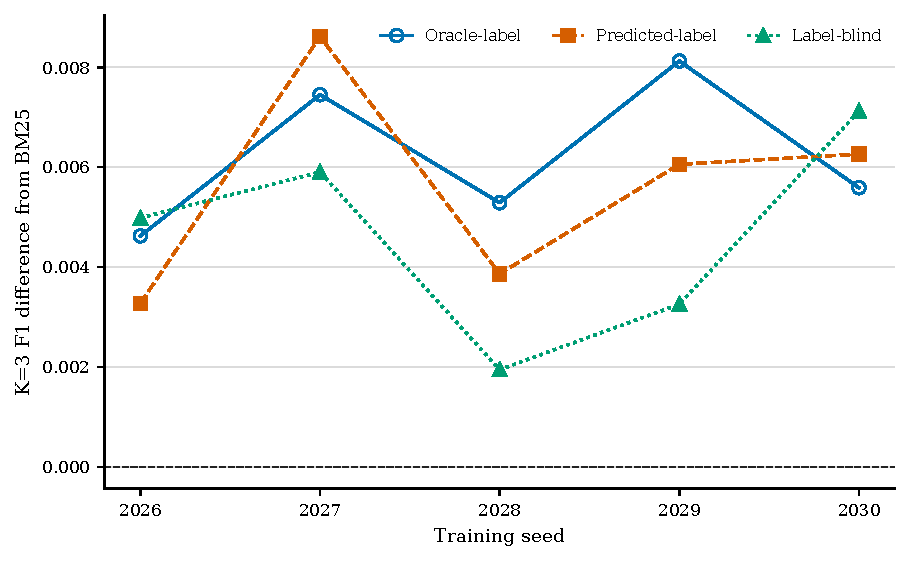
\includegraphics[width=0.92\textwidth]{figures/results/fig04_seed_stability_k3.pdf}
\caption{Per-seed primary-budget difference from fixed BM25, including the pilot seed. No test-based seed selection is applied.}\label{fig:seed}
\end{figure}

\begin{figure}[H]
\centering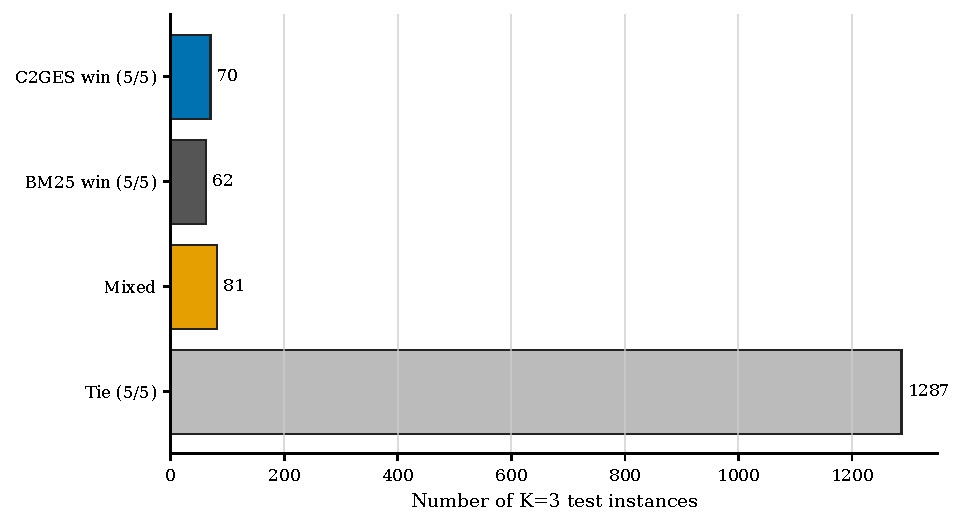
\includegraphics[width=0.86\textwidth]{figures/results/fig05_k3_case_stability.pdf}
\caption{Instance-level predicted-label outcomes against BM25 across seeds. Categories use sentence-ID F1 outcomes and are not semantic error labels.}\label{fig:cases}
\end{figure}

The seed-stability figure makes model variation visible instead of reporting only the best run. At the primary budget, learned-system differences from BM25 vary across seeds even though the aggregate predicted-label gate is positive. This variation motivates retaining checkpoints and seed-level rows and cautions against publishing a result selected after test inspection. The figure is paired to the same deterministic BM25 row for every seed, so its vertical movement reflects the learned reranker rather than baseline randomness.

The case-stability analysis classifies all \CaseCount{} test instances solely by sentence-ID F1 outcomes over the frozen seeds. Of these, \CaseAllTie{} are tied in every seed under the category definition. Remaining categories distinguish consistent wins, consistent losses, and seed-dependent outcomes. These categories identify where manual analysis may be useful, but they are not semantic labels such as ``lexical failure'' or ``causal success.'' Assigning such explanations requires reading source sentences and should be independently reviewed rather than inferred from score deltas.

\subsection{Qualitative Power-Grid Workflow}
The NERC material is used to specify how the method would enter a reliability-report workflow. A reviewer begins with a question scoped to a role such as initiating event, root cause, propagation or response, impact, or mitigation. The document parser produces stable sentence identifiers; the selector then returns a short packet with component scores and role provenance. A reviewer can accept, reject, or supplement the packet while retaining a link to the official source report.

This workflow differs from autonomous causal diagnosis. \cges{} does not infer grid topology, reconstruct a disturbance sequence from measurements, or establish that one event caused another. It ranks textual candidates. A high local-chain score indicates proximity to other relevant text, and a high role score indicates model compatibility with an input label. Neither is a substitute for engineering judgment or corroborating operational data.

The NERC annotation study contains two disjoint 15-document sets, each with five role-conditioned questions per document. The 75-item development set was visible while the protocol was refined. The second 75-item packet was assembled and hash-frozen before annotation, excluded all development documents, retained stable sentence identifiers, and exposed no reference evidence to an annotator. Annotators A and B labelled answerability, evidence role, and evidence identifiers independently. Deterministic Tier-1 rules resolved granularity differences such as subset-minimal and intersection consensus; only substantive Tier-2 disagreements were sent to annotator C.

On development, answerability and role agreement were both 0.853, evidence-set Jaccard was 0.599, and 25/75 items (0.333) required Tier-2 machine adjudication. On the frozen set, answerability and role agreement were 0.973, evidence-set Jaccard was 0.631, and 13/75 items (0.173) required Tier-2 adjudication. Both stages ended with zero unresolved items and zero format/API failures. Exact evidence-set agreement remained only 0.413 and 0.240, respectively, showing that high answerability agreement does not eliminate span-granularity differences. These are annotation-process statistics, not selector accuracy.

The resulting records can reveal parsing problems, broken identifiers, unclear roles, and annotation-granularity risk. They cannot provide a defensible domain F1 value or establish improvement over a baseline because every final label remains machine-adjudicated silver. For this reason the manuscript includes no NERC leaderboard or selected model-performance result.

A future expert validation can reuse the tested separation between development and frozen packets, but qualified human annotators must independently select evidence without seeing model outputs or silver labels. Disagreements must be retained and adjudicated under a documented manual. Only after that human evidence tier, the selector, and the analysis plan are frozen should domain performance be scored. This sequence keeps model-assisted annotation from becoming circular evidence for the same model.

\section{Discussion}
Document-grouped splitting, out-of-fold role construction, and explicit oracle labeling make the evaluation auditable. Under that protocol, predicted-label \cges{} shows a small positive comparison with BM25 at moderate evidence budgets, while BM25 remains better at the smallest budget. The result illustrates a budget-dependent benchmark trade-off rather than a general advantage for either method.

\subsection{Supported Interpretation}
The strongest supported contribution is methodological transparency. The study exposes how documents are partitioned, how role labels are obtained, where gold data enter, how uncertainty respects source clustering, and how every table connects to immutable predictions. The resulting evidence does not support a role-driven gain; it supports an auditable reranker whose relative behavior depends on the output budget.

Evidence-selection systems are commonly evaluated under different output budgets because a single returned sentence and a short evidence packet impose different precision--recall trade-offs. In the present benchmark, BM25 is competitive at the smallest budget, whereas the mixed reranker is a candidate for target-domain validation when a larger packet is acceptable. The observed differences are modest and do not establish utility in technical-report review.

Interpretability here has a precise, limited meaning: the final score is decomposable, candidate identifiers are retained, and role provenance is visible. It does not mean that individual components are causal explanations of model behavior, that the role head corresponds to human reasoning, or that a selected sentence is factually correct outside the FEVER annotation. This distinction is especially important in reliability analysis, where explanatory language can be mistaken for physical causation.

The role mechanism itself is not supported by the predefined primary contrast. Predicted-label and label-blind results are practically close, and their uncertainty intervals cross zero. This finding rules out statements that the role head is the source of the observed moderate-budget advantage. Plausible explanations include limited information in binary FEVER roles, upstream classification error, and mixture floors that constrain the label-blind and role-aware solutions similarly. These are hypotheses for new experiments, not post hoc conclusions.

The crossed seed matrix reduces concern that one fixed upstream ledger dominates full-model variability. Across the five upstream fits tested, upstream marginal variation was smaller than downstream marginal variation and the nonnegative method-of-moments estimate for the upstream component was zero. Interaction/residual variation remained, and the document-composition range was much wider than either seed-marginal range. This sensitivity analysis does not re-estimate the role effect because it does not retrain a label-blind comparator; it remains conditional on this classifier, corpus, and finite seed set.

The oracle protocol provides a sensitivity analysis only. Its proximity to end-to-end protocols suggests that access to the gold veracity label does not create a large measured advantage here, but the result cannot be deployed because veracity is unavailable at selection time. The study also does not establish open-corpus retrieval quality: the correct source document is supplied, and only sentences within it are ranked.

\subsection{Implications for Model Development}
The unsupported role effect indicates that simply increasing the seed count around the same binary role and constrained mixture would not address the underlying ambiguity. More informative tests include a query-only learned selector, a role-head removal that also removes its floor, a no-floor mixture, and role labels aligned with domain information needs rather than FEVER veracity. Each should preserve the document split and paired evaluation so that improvements cannot be attributed to easier candidates.

The two cross-encoder evaluations provide contemporary interaction-reranker references on identical sentence pools under frozen snapshots, but they do not establish an accuracy--cost frontier. Their runtime boundaries differ from learned-system training, and neither comparison family produced a Holm-adjusted finding. BGE was statistically unresolved against full \cges{} and BM25 under the prespecified randomization criterion, while its negative point contrast against MiniLM also failed that criterion after adjustment. Additional rerankers and neural listwise methods remain useful replication targets. Reporting only accuracy would be insufficient for a technical-report tool: throughput, peak memory, model size, offline encoding, and trace availability should accompany each comparison.

The result also illustrates the value of negative evidence in applied machine learning. A failed component hypothesis prevents an organization from treating a semantically appealing feature as validated. Preserving the negative result, source ledger, and decision criterion makes subsequent changes comparable and reduces the temptation to rename a post hoc pattern as the original contribution.

\subsection{Limitations and Planned Validation}
The seed sample is small; all five seeds are reported, including the pilot run that preceded the four-seed prospective continuation. Hierarchical resampling captures seed and document variation but does not cover distribution shift to new corpora. Exact document disjointness does not exclude redirect aliases or semantic near-duplicates. The local channel is positional smoothing rather than causal structure, and the resource monitor does not measure GPU memory or sub-sampling-interval peaks.

The power-grid application remains unvalidated at the selector-performance level. The local NERC development and frozen sets have complete machine-adjudicated silver labels and useful agreement diagnostics, but they do not constitute an independently adjudicated human-gold benchmark. A quantitative domain study requires a frozen manual, multiple independent domain reviewers, recorded disagreements, human adjudication, agreement statistics, and a sealed test subset whose silver labels are hidden during expert review. Until that evidence is available, no NERC selector-performance value can be reported.

Additional limitations follow from the metric and corpus. FEVER may provide incomplete evidence sets, and exact sentence-ID F1 does not grade semantic adequacy or the usefulness of a packet to an engineer. The binary SUPPORTS/REFUTES role is much coarser than the causal and operational categories implied by reliability-report review. The benchmark supplies a source document, so page retrieval errors, OCR quality, report segmentation, tables, figures, and multi-document evidence are outside scope.

External validity is also limited by genre. Wikipedia prose is comparatively regular and differs from incident narratives, recommendations, appendices, and tabular event chronologies. A model that is auditable on FEVER may still fail on long reports, scanned PDFs, or domain abbreviations. The Featured Application and Introduction communicate the intended use, while the abstract and data section explicitly identify the quantitative corpus to prevent that goal from being mistaken for completed domain validation.

Finally, reproducibility artifacts do not eliminate governance obligations. FEVER licensing and attribution must accompany any redistributed conversion. Public availability of a NERC PDF does not automatically authorize redistribution of extracted text, and automatically constructed annotations must retain their machine provenance. The release package must therefore separate redistributable code and derived statistics from source text whose redistribution has not been confirmed.

\section{Conclusions}
This study evaluates \cges{} under a leakage-controlled three-protocol design. The five-seed results, comprising one pilot and four prospectively specified continuation seeds, show budget-dependent behavior relative to BM25 but no reliable gain from predicted role conditioning over the label-blind system. A finite exploratory analysis reports all nine existing modes, while separately specified experiments retrain true no-floor and true no-role variants and evaluate frozen MiniLM and BGE cross-encoders. Neither cross-encoder comparison family produced a Holm-adjusted finding, and the floor-removal variants do not support a positive claim. A crossed 25-pipeline sensitivity study found less marginal variation across the five upstream fits than across the five downstream fits, without changing the role-effect conclusion. The NERC study establishes a hash-frozen, zero-unresolved machine-silver annotation workflow and quantifies its remaining evidence-granularity disagreement; it does not establish selector accuracy on power-grid reports. The supported contribution is a traceable evidence-selection method, an explicit role-provenance evaluation, and a bounded path from machine-silver development data to future independently adjudicated domain evidence.

\supplementary{The reproducibility package contains executable source and hashes, the frozen split manifest, conversion audit, upstream-role provenance, the serialized role model, all 15 main-study downstream configurations and checkpoints, complete prediction ledgers, tabular results, figures, environment records, and verification scripts. It also includes the BGE protocol, exact model-file inventory and revision, 6,000-row prediction ledger, resource and provenance records, primary contrast table, and independent numerical validation report. The crossed seed-sensitivity package adds five upstream artifacts, 25 downstream ledgers, 450,000 selected analysis rows, its fixed analysis specification, cell summary, and validation record. The NERC package adds separate 75-item development and frozen packets, per-document and set hashes, independent model labels, deterministic-resolution records, adjudication ledgers, and statistics; every record retains explicit machine-silver provenance. Public project code and license-cleared materials are available at \url{https://github.com/gaoxingkele/c2ges}; the exact submission-version verification package is also available from the corresponding author upon reasonable request.}
\authorcontributions{Conceptualization, B.L. and Y.Y.; methodology, B.L.; software, B.L.; validation, B.L.; formal analysis, B.L.; investigation, B.L.; resources, Y.Y.; data curation, B.L.; writing---original draft preparation, B.L.; writing---review and editing, B.L. and Y.Y.; visualization, B.L.; supervision, Y.Y.; project administration, Y.Y.; funding acquisition, Y.Y. All authors have read and agreed to the published version of the manuscript.}
\funding{This research was funded by the Science and Technology Project of NARI Group Corporation (State Grid Electric Power Research Institute), grant number 521300250006.}
\institutionalreview{Not applicable. This study did not involve humans or animals; it uses a public human-annotated benchmark and public technical reports.}
\informedconsent{Not applicable.}
\dataavailability{FEVER is available from its original providers \cite{thorne2018fever}, and public project code and license-cleared reproducibility materials are available at \url{https://github.com/gaoxingkele/c2ges}. The original Hugging Face source revision was not recorded; the retained cache fingerprints and converted-file hashes are reported instead. Owing to third-party licensing restrictions, the NERC source documents and any submission-version materials not included in the public repository are available from the corresponding author upon reasonable request for editorial and peer-review verification, subject to third-party permission and the applicable licenses. The request package contains the document-grouped split manifest, conversion and audit code, main and crossed-seed upstream artifacts, downstream run configurations and predictions, statistical outputs, verification scripts, and the development and frozen NERC machine-silver annotation records.}
\acknowledgments{During preparation of this manuscript, the authors used OpenAI Codex (GPT-5-based) for drafting, editing, code review, and reproducibility checks. DeepSeek, Gemini, and GPT-based services were used as machine annotators or adjudicator for the NERC silver-label study. The authors reviewed and edited the outputs and take full responsibility for the content of the publication. Machine-adjudicated NERC labels are not presented as human or domain-expert ground truth and are not used for selector-performance claims.}
\conflictsofinterest{The authors declare no conflicts of interest. The funder had no role in the design of the study; in the collection, analyses, or interpretation of data; in the writing of the manuscript; or in the decision to publish the results.}

\begin{adjustwidth}{-\extralength}{0cm}
\reftitle{References}
\bibliography{references_cited_verified}
\PublishersNote{}
\end{adjustwidth}
\end{document}
